\documentclass{beamer}
\usepackage[utf8]{inputenc}

\usetheme{Madrid}
\usecolortheme{default}
\usepackage{amsmath,amssymb,amsfonts,amsthm}
\usepackage{txfonts}
\usepackage{tkz-euclide}
\usepackage{listings}
\usepackage{adjustbox}
\usepackage{array}
\usepackage{tabularx}
\usepackage{gvv}
\usepackage{lmodern}
\usepackage{circuitikz}
\usepackage{tikz}
\usepackage{graphicx}

\setbeamertemplate{page number in head/foot}[totalframenumber]

\usepackage{tcolorbox}
\tcbuselibrary{minted,breakable,xparse,skins}



\definecolor{bg}{gray}{0.95}
\DeclareTCBListing{mintedbox}{O{}m!O{}}{%
  breakable=true,
  listing engine=minted,
  listing only,
  minted language=#2,
  minted style=default,
  minted options={%
    linenos,
    gobble=0,
    breaklines=true,
    breakafter=,,
    fontsize=\small,
    numbersep=8pt,
    #1},
  boxsep=0pt,
  left skip=0pt,
  right skip=0pt,
  left=25pt,
  right=0pt,
  top=3pt,
  bottom=3pt,
  arc=5pt,
  leftrule=0pt,
  rightrule=0pt,
  bottomrule=2pt,
  toprule=2pt,
  colback=bg,
  colframe=orange!70,
  enhanced,
  overlay={%
    \begin{tcbclipinterior}
    \fill[orange!20!white] (frame.south west) rectangle ([xshift=20pt]frame.north west);
    \end{tcbclipinterior}},
  #3,
}
\lstset{
    language=C,
    basicstyle=\ttfamily\small,
    keywordstyle=\color{blue},
    stringstyle=\color{orange},
    commentstyle=\color{green!60!black},
    numbers=left,
    numberstyle=\tiny\color{gray},
    breaklines=true,
    showstringspaces=false,
}
%------------------------------------------------------------
%This block of code defines the information to appear in the
%Title page
\title %optional
{1.5.36}
\date{}
%\subtitle{A short story}

\author % (optional)
{Sai Krishna Bakki - EE25BTECH11049}



\begin{document}


\frame{\titlepage}
\begin{frame}{Question}
Find the unit vector in the direction of the  vector ${a} = \hat{i} + \hat{j} + 2\hat{k}$ 
\end{frame}

\begin{frame}{Theoretical Solution}
Given 
\begin{align}
\vec{A}= \myvec{1 \\ 1 \\2 }
\end{align}
\begin{align}
    {||\vec{a}||} =\sqrt{\vec{a}^\top\vec{a}}=\sqrt{\brak{1}^2+\brak{1}^2+\brak{2}^2}=\sqrt{6}
\end{align}
The unit vector in the direction of $\vec{a}$ is 
\begin{align}
    \frac{\vec{a}}{||\vec{a}||}=\frac{1}{\sqrt{6}}\myvec{1\\1\\2}
\end{align}
\end{frame}
\begin{frame}[fragile]
\frametitle{C Code }
\begin{lstlisting}
#include <stdio.h>
#include <math.h>


// Function to calculate the unit vector.
// It takes an input vector, its size, and an output array for the result.
void calculate_unit_vector_c(double *vector, int size, double *unit_vector_out) {
    double magnitude = 0.0;
    int i;

    // Calculate the magnitude of the vector
    for (i = 0; i < size; i++) {
        magnitude += vector[i] * vector[i];
    }
    magnitude = sqrt(magnitude);
\end{lstlisting}
\end{frame}  

\begin{frame}[fragile]
\frametitle{C Code }
\begin{lstlisting}

    // To avoid division by zero, if magnitude is 0, return a zero vector.
    if (magnitude == 0) {
        for (i = 0; i < size; i++) {
            unit_vector_out[i] = 0.0;
        }
    } else {
        // Calculate the unit vector
        for (i = 0; i < size; i++) {
            unit_vector_out[i] = vector[i] / magnitude;
        }
    }
}
\end{lstlisting}
\end{frame}  

\begin{frame}[fragile]
\frametitle{Python Code through shared output}
\begin{lstlisting}
import numpy as np
import matplotlib.pyplot as plt
from mpl_toolkits.mplot3d import Axes3D
import ctypes
from numpy.ctypeslib import ndpointer

# This script uses the compiled C library 'vector_lib.so' 
# to calculate the unit vector.
#
# Before running this script, you must compile the C code by running
# the following command in your terminal:
# python setup.py build_ext --inplace

try:
    # --- 1. Load the C Shared Library ---
    # This loads the .so (Linux/macOS) or .dll (Windows) file.
    vector_lib = ctypes.CDLL('./vector_lib.so') 
    \end{lstlisting}
\end{frame}  

\begin{frame}[fragile]
\frametitle{Python Code through shared output}
\begin{lstlisting}
    
    # --- 2. Define the C function's argument and return types ---
    # This tells Python how to correctly call the C function.
    calculate_unit_vector_c = vector_lib.calculate_unit_vector_c
    calculate_unit_vector_c.restype = None  # The C function returns void
    calculate_unit_vector_c.argtypes = [
        ndpointer(dtype=np.float64, flags="C_CONTIGUOUS"), # Pointer to the input vector
        ctypes.c_int,                                     # Integer for the vector size
        ndpointer(dtype=np.float64, flags="C_CONTIGUOUS")  # Pointer to the output array
    ]

    # --- 3. Prepare data and call the C function ---
    from params import a_vector
    \end{lstlisting}
\end{frame}  

\begin{frame}[fragile]
\frametitle{Python Code through shared output}
\begin{lstlisting}
    
    # Ensure the vector is a float64 numpy array for the C function
    a = a_vector.astype(np.float64)
    
    # Create an empty numpy array to store the result from C
    unit_a = np.zeros_like(a, dtype=np.float64)

    # Call the C function
    calculate_unit_vector_c(a, a.size, unit_a)

    # --- 4. Print and Plot the results ---
    magnitude_a = np.linalg.norm(a) # Calculate magnitude in Python for display
    \end{lstlisting}
\end{frame}  

\begin{frame}[fragile]
\frametitle{Python Code through shared output}
\begin{lstlisting}

    print(f"Original vector a: {a}")
    print(f"Magnitude of a: {magnitude_a:.4f}")
    print(f"Unit vector â (from C library): {unit_a}")
    print(f"Magnitude of the unit vector: {np.linalg.norm(unit_a):.4f}")
    

    # Create the 3D plot
    fig = plt.figure(figsize=(10, 10))
    ax = fig.add_subplot(111, projection='3d')

    # Plot the original vector 'a' and the unit vector 'â'
    ax.quiver(0, 0, 0, a[0], a[1], a[2], color='b', arrow_length_ratio=0.1, label=f'Vector a = {a}')
    ax.quiver(0, 0, 0, unit_a[0], unit_a[1], unit_a[2], color='r', arrow_length_ratio=0.2, label=f'Unit Vector â ≈ [{unit_a[0]:.2f}, {unit_a[1]:.2f}, {unit_a[2]:.2f}]')
\end{lstlisting}
\end{frame}  

\begin{frame}[fragile]
\frametitle{Python Code through shared output}
\begin{lstlisting}
    # Configure and display the plot
    limit = max(np.max(np.abs(a)), 1.5)
    ax.set_xlim([-limit, limit]); ax.set_ylim([-limit, limit]); ax.set_zlim([0, limit])
    ax.set_title('Unit Vector in 3D (Calculated in C)', fontsize=16)
    ax.set_xlabel('x-axis'); ax.set_ylabel('y-axis'); ax.set_zlabel('z-axis')
    ax.legend(fontsize=12)
    ax.view_init(elev=20., azim=30)
    plt.grid(True)
    plt.show()
    \end{lstlisting}
\end{frame}  

\begin{frame}[fragile]
\frametitle{Python Code through shared output}
\begin{lstlisting}

except FileNotFoundError:
    print("Error: Could not find 'vector_lib.so' or 'vector_lib.dll'.")
    print("Please ensure you have compiled the C library first by running this command in your terminal:")
    print("python setup.py build_ext --inplace")
except Exception as e:
    print(f"An unexpected error occurred: {e}")

\end{lstlisting}
\end{frame}  

\begin{frame}[fragile]
\frametitle{Python Code}
\begin{lstlisting}
import numpy as np
import matplotlib.pyplot as plt
from mpl_toolkits.mplot3d import Axes3D
from funcs import calculate_unit_vector
from params import a_vector # Import the specific vector

# The vector a = (1, 1, 2) is now defined in params.py
# This script calculates its unit vector and creates a 3D plot for visualization.

try:
    # Calculate the unit vector using the function from funcs.py
    a, magnitude_a, unit_a = calculate_unit_vector(a_vector)

    # Print the results
    print(f"Original vector a: {a}")
    print(f"Magnitude of a: {magnitude_a:.4f}")
    print(f"Unit vector â: {unit_a}")
    \end{lstlisting}
\end{frame}

\begin{frame}[fragile]
\frametitle{Python Code}
\begin{lstlisting}
    print(f"Magnitude of the unit vector: {np.linalg.norm(unit_a):.4f}")


    # --- Plotting the Vectors ---

    # Create the 3D plot
    fig = plt.figure(figsize=(10, 10))
    ax = fig.add_subplot(111, projection='3d')

    # Plot the original vector 'a' in blue
    ax.quiver(0, 0, 0, a[0], a[1], a[2], color='b', arrow_length_ratio=0.1, label=f'Vector a = {a}')

    # Plot the unit vector 'â' in red
    ax.quiver(0, 0, 0, unit_a[0], unit_a[1], unit_a[2], color='r', arrow_length_ratio=0.2, label=f'Unit Vector â ≈ [{unit_a[0]:.2f}, {unit_a[1]:.2f}, {unit_a[2]:.2f}]')
    \end{lstlisting}
\end{frame}

\begin{frame}[fragile]
\frametitle{Python Code}
\begin{lstlisting}

    # Set the plot limits for better visualization
    limit = max(np.max(np.abs(a)), 1.5)
    ax.set_xlim([-limit, limit])
    ax.set_ylim([-limit, limit])
    ax.set_zlim([0, limit])

    # Set plot title and labels
    ax.set_title('Unit Vector in 3D', fontsize=16)
    ax.set_xlabel('x-axis', fontsize=12)
    ax.set_ylabel('y-axis', fontsize=12)
    ax.set_zlabel('z-axis', fontsize=12)

    # Add a legend
    ax.legend(fontsize=12)

    # Set the view angle
    ax.view_init(elev=20., azim=30)
    \end{lstlisting}
\end{frame}

\begin{frame}[fragile]
\frametitle{Python Code}
\begin{lstlisting}

    # Display the plot
    plt.show()

except (ValueError, NameError) as e:
    print(f"An error occurred: {e}")
    print("Please ensure that 'params.py' contains 'a_vector' and 'funcs.py' contains 'calculate_unit_vector'.")


\end{lstlisting}
\end{frame}

\begin{frame}{Plot by python using shared output from c}
	\begin{center}
		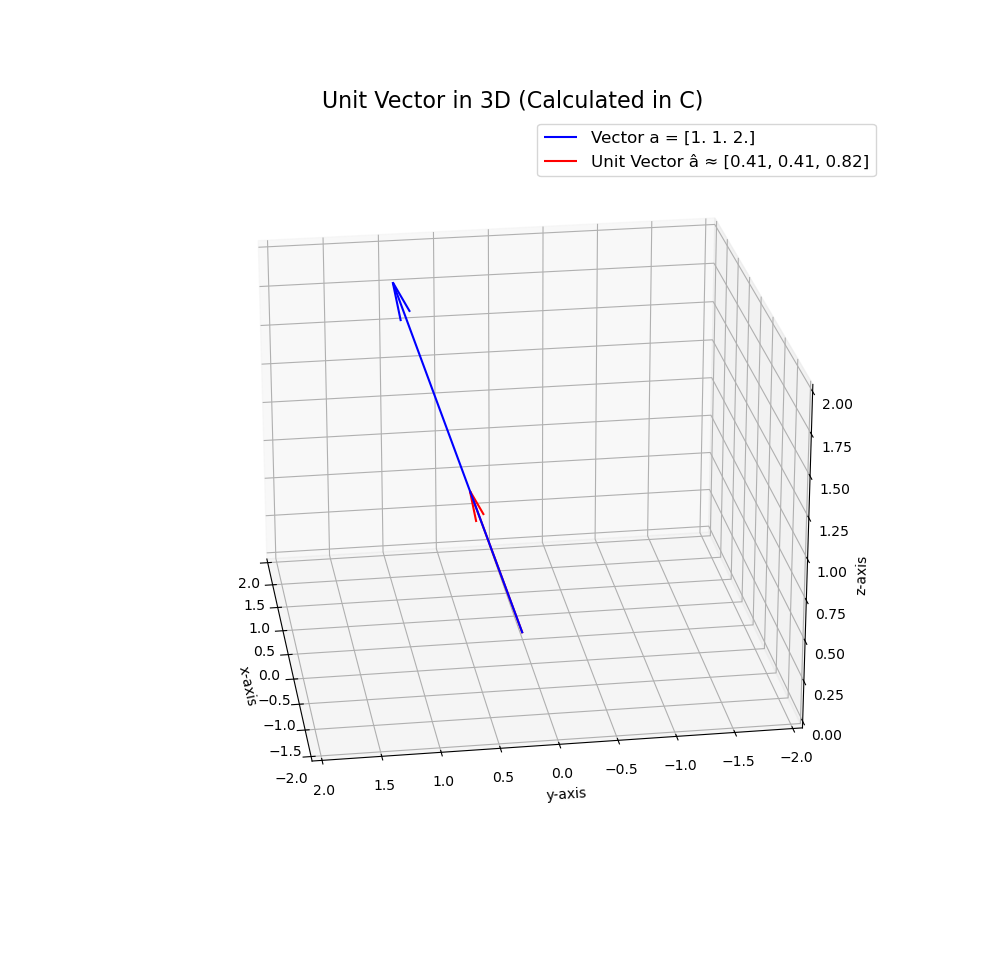
\includegraphics[width=0.6\columnwidth]{figs/Figure.png}
	\end{center}
\end{frame}
\begin{frame}{Plot by using Python only}
	\begin{center}
		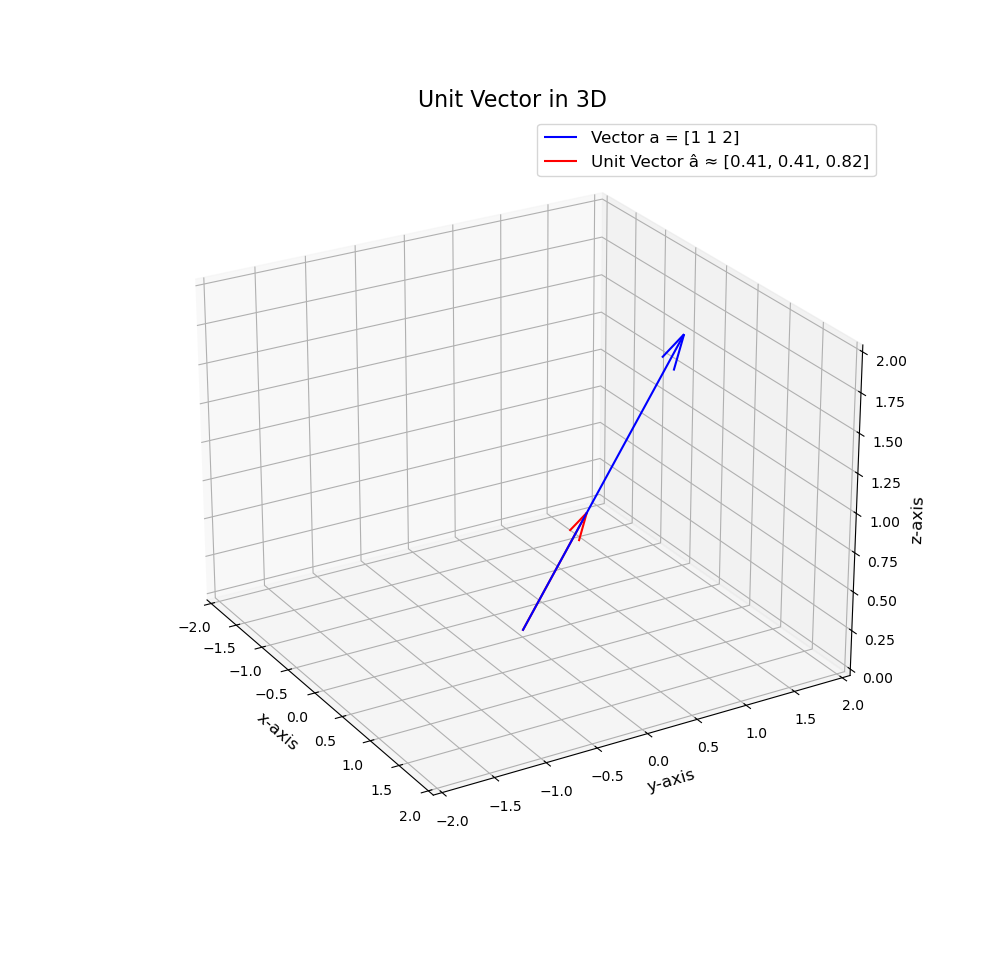
\includegraphics[width=0.6\columnwidth]{figs/Figure_1.png}
	\end{center}
\end{frame}
\end{document}
